
\noindent{\bf 1. Introduction.} Time series and spatial statistics with Noel Cressie's results \\

%%------------------------------------------------------------------%%
\section{Random process on a circle}
%%------------------------------------------------------------------%%

Let $X(t)$ be the random process on the unit circle $S^1$. If $X(t)$ is further assumed to be with finite second moment and continuity in quadratic mean, then $X(t)$ can be represented in a Fourier series which is convergent in quadratic mean (\cite{DUFOUR1976107}),
\[
X(t) = A_0 + \sum_{n=1}^\infty (A_n\cos(nt) + B_n \sin(nt)), \quad \quad t \in S^1,
\]
where
\begin{eqnarray*}
A_0 = \frac{1}{2\pi}\int_S X(t)dt, \quad A_n = \frac{1}{\pi}\int_S X(t)\cos(nt)dt, \quad B_n = \frac{1}{\pi}\int_S X(t)\sin(nt)dt.
\end{eqnarray*}

Let $s, t \in S^1$. The covariance function $C(s, t)$ of the process $X(t)$ on the given locations $s$ and $t$ is given below
\begin{eqnarray*}
C(s, t) = cov(X(s), X(t)).
\end{eqnarray*}
Now we assume the underlying process $X(t)$ is stationary on the circle, that is, $E(X(t)) = \mu$ unknown, and its covariance function solely depends on the angular distance $\theta$
\[
C(\theta) = cov(X(t+\theta), X(t)), \quad \quad \theta \in [0, \pi].
\]
Under the assumption of stationarity, we have
\begin{eqnarray*}
cov(A_n, A_m) = cov(B_n, B_m) = a_n \delta(n, m), \quad \quad \mbox{and} \quad \quad cov(A_n, B_m) = 0, \quad \mbox{for $n \ge 0, m > 0$},
\end{eqnarray*}
with $a_n \ge 0$, under which the covariance function $C(\theta)$ can be written as the following spectral representation
\begin{eqnarray*}
C(\theta) = a_0 + \sum_{n=1}^\infty a_n \cos(n\theta), \quad \quad \mbox{for $\theta \in [0, \pi]$}.
\end{eqnarray*}
By the orthogonality of $\{\cos(n\theta), n = 0, 1, 2, \cdots,\}$ on $\theta \in [0, \pi]$, we have
\[
a_0 = \frac{1}{\pi}\int_0^\pi C(\theta)d\theta, \quad \quad a_n = \frac{2}{\pi}\int_0^\pi C(\theta)\cos(n\theta)d\theta, \quad n \ge 1.
\]
If a random process $X(t)$ is intrinsically stationary, one has $E(X(t)) = \mu$, an unknown constant, as well as the variogram function depends only on the angular distance $\theta$, given by
\begin{eqnarray*}
\gamma(\theta) = var(X(t+\theta) - X(t)), \quad \quad t \in S^1.
\end{eqnarray*}
Note that if $X(t)$ is stationary, then
\[
\gamma(\theta) = C(0) - C(\theta).
\]
Equivalently, $\gamma(\theta)$ has the following spectral representation
\[
\gamma(\theta) = \sum_{n = 1}^\infty a_n (1 - \cos(n\theta)).
\]

%-------------------------------------%
\subsection{Mean and covariance estimation on the circle}
%-------------------------------------%

The ultimate goal in the spatial statistics is to make prediction of random process on the unobserved location. We now consider the estimation on the unknown mean $\mu$ and covariance function $C(\theta)$. Let $\{X(t_k), k = 1, 2, \cdots, n\}$ be a collection of gridded observations on the unit circle, with $t_k = (k-1)*2\pi/n, k = 1, 2, \cdots, n$. For simplicity, let $n = 2N$ be an even number. Denote $\utilde{X} = (X_1, X_2, \cdots, X_n)^T$ as the observed random vector. When the underlying process $X(t)$ is stationary on the unit circle, the variance-covariance matrix of $\utilde{X}$ is given by

% \begin{eqnarray*}
% \Sigma &=& \left(\begin{array}{cccccccccc}
% C(0)      & C(2\pi/n) & \cdots & C((N-1)2\pi/n) & C(\pi) &  C((N-1)2\pi/n) & \cdots & C(2\pi/n) \\
% C(2\pi/n) & C(0)  & \cdots & C((N-2)2\pi/n) & C((N-1)2\pi/n) &  C(\pi)  & \cdots & C(4\pi/n) \\
% C(4\pi/n) & C(2\pi/n)  & \cdots & C((N-3)2\pi/n) & C((N-2)2\pi/n) &  C((N-1)2\pi/n) & \cdots & C(6\pi/n) \\
% \vdots    &    \vdots  & \vdots  & \vdots  & \vdots  & \vdots  & \vdots  & \vdots  \\
% C(2\pi/n) & C(4\pi/n)& \cdots & C(\pi) &  C((N-1)2\pi/n) & C((N-2)2\pi/n)  & \cdots & C(0)
% \end{array}
% \right) \\
% &=& circ(C(0),C(2\pi/n), C(4\pi/n), \cdots, C((N-1)2\pi/n), C(\pi),  C((N-1)2\pi/n), \cdots, C(2\pi/n)),
% \end{eqnarray*}

\begin{eqnarray*}
	\Sigma &=& \left(\begin{array}{ccccccc}
	C(0)      & \cdots & C((N-1)\delta ) & C(\pi) &  C((N-1)\delta ) & \cdots & C(\delta) \\
	C(\delta) & \cdots & C((N-2)\delta) & C((N-1)\delta) &  C(\pi)  & \cdots & C(2\delta) \\
	C(2\delta) & \cdots & C((N-3)\delta) & C((N-2)\delta) &  C((N-1)\delta) & \cdots & C(3\delta)\\
	\vdots    & \vdots  & \vdots  & \vdots  & \vdots  & \vdots  & \vdots  \\
	C(\delta) & \cdots & C(\pi) &  C((N-1)\delta) & C((N-2)\delta)  & \cdots & C(0) 
	\end{array} \right),
\end{eqnarray*}

is a symmetric circulant matrix with elements $C(0),C(\delta), C(2\delta), \cdots, C((N-1)\delta), C(\pi),  C((N-1)\delta), \cdots, C(\delta)$ where $\delta = 2\pi/n$. Therefore the sample mean
\[
\bar{X} = \frac{1}{n}{\bf 1}_n^T \utilde{X}
\]
is an unbiased estimator of $\mu$ with the variance given by

\begin{eqnarray*}
var(\bar{X}) &=& cov(\frac{1}{n}{\bf 1}_n^T \utilde{X}, \frac{1}{n}{\bf 1}_n^T \utilde{X}) \nonumber \\
	&=& \frac{1}{n^2}{\bf 1}_n^T \Sigma {\bf 1}_n \nonumber \\
	&=& \frac{1}{n} \left(C(0)+C(\pi)+2 \sum_{m=1}^{N-1}C(m 2\pi/n)\right) \nonumber
\end{eqnarray*}

If we assume that $C(\theta)$ is a continuous function on $[0, \pi]$ and note the summation in the last quantity is a trapezoid sum of $C(\theta)$ on the gridded locations within $[0, \pi]$, then,

\[
\frac{1}{\pi} \frac{\pi}{2 N} \left(C(0) + \sum_{m=1}^{N-1}C(m 2\pi/n) + C(\pi) \right) \to \frac{1}{\pi} \int_0^\pi C(\theta)d\theta = a_0,
\]
as $n \to \infty$. That is, $var(\bar{X}) \to a_0$ as $n \to \infty$. Therefore, we have the following proposition. \\

\begin{prop} \label{prop3.1}

The sample mean $\bar{X}$ is an unbiased estimator of $\mu$ with the asymptotic variance of $a_0$. If $a_0 > 0$ and $X(t)$ is further assumed to be Gaussian, then $\bar{X}$ is NOT a consistent estimator of $\mu$. \\

{\bf Proof:} It is only necessary to prove the second part. If $X(t)$ is Gaussian, then $\bar{X} \sim N(\mu, var(\bar{X})) \Rightarrow Z = \frac{\bar{X} - \mu}{\sqrt{var(\bar{X})}} \sim N(0, 1)$. First, for a fixed $\varepsilon_0 > 0$ and $\varepsilon_0 < a_0$, there exists $K$, such that for all $n > K$, we have
\[
|var(\bar{X}) - a_0| < \varepsilon_0 \Rightarrow a_0 - \varepsilon_0 < var(\bar{X}) < a_0 + \varepsilon_0.
\]
Now for each fixed $\varepsilon > 0$ and all $n > K$,
\begin{eqnarray*}
P\left(|\bar{X} - \mu| > \varepsilon\right) &=& P\left(\frac{|\bar{X} - \mu|}{\sqrt{var(\bar{X})}} > \frac{\varepsilon}{\sqrt{var(\bar{X})}} \right) \\
&\ge& P\left(|Z| > \frac{\varepsilon}{\sqrt{a_0 - \varepsilon_0}} \right) > 0.
\end{eqnarray*}
Hence $\bar{X} \not\to \mu$ in probability. The last inequality above is due to the following.

\[
\left\{|Z| > \frac{\varepsilon}{\sqrt{a_0 - \varepsilon_0}} \right\} \subseteq \left\{|Z| > \frac{\varepsilon}{\sqrt{var(\bar{X})}}\right\}.
\]

\end{prop}

\vskip 8pt

Now we consider the MOM estimator of $C(\theta)$, given by

\beq \label{covarince_estimator}
\hat{C}(\Delta \lambda) = \frac{1}{n}\sum_{i = 1}^n (X(t_i + \Delta \lambda) - \bar{X})(X(t_i) - \bar{X}), 
\eeq

where $\Delta \lambda = 0, 2\pi/n, 4\pi/n, \cdots, 2(N-1)\pi/n$.\\

Now we calculate the unbiasedness and consistency of the above estimator.

\begin{eqnarray*}
	E(\hat{C}(\Delta \lambda)) &=& \frac{1}{n}\sum_{i = 1}^n E((X(t_i + \Delta \lambda) - \bar{X})(X(t_i) - \bar{X})) \\ 
	&=& \frac{1}{n}\sum_{i = 1}^n E((X(t_i + \Delta \lambda) - \mu - (\bar{X} - \mu))(X(t_i) -\mu - (\bar{X}) - \mu)) \\ 
	&=& \frac{1}{n}\sum_{i=1}^n cov(X(t_i+\Delta \lambda), X(t_i)) - \frac{1}{n}\sum_{i = 1}^n E((X(t_i + \Delta \lambda) - \mu)(\bar{X} - \mu)) \\ 
	& & -\frac{1}{n}\sum_{i = 1}^n E((X(t_i) - \mu)(\bar{X} - \mu)) + \frac{1}{n}\sum_{i = 1}^n E((\bar{X} - \mu)(\bar{X} - \mu)) \\ 
	&=& C(\Delta \lambda) -E((\bar{X} - \mu)(\bar{X} - \mu)) - E((\bar{X} - \mu)(\bar{X} - \mu)) \\  
	& & + E((\bar{X} - \mu)(\bar{X} - \mu)) \\ 
	&=& C(\Delta \lambda) - var(\bar{X}).
\end{eqnarray*}

That is, the MOM estimator $\hat{C}(\Delta \lambda)$ of the covariance function is actually a biased estimator with the shift amount approximately equal to $a_0$ unless $a_0 = 0$. In other words, if $a_0 = 0$, the MOM estimator $\hat{C}(\Delta \lambda)$ is an unbiased estimator of $C(\theta)$. In summary, we have \\

\begin{prop} \label{prop3.2}
The MOM covariance estimator is a biased estimator of the true covariance function $C(\theta)$, if $a_0 > 0$. However, if the process is a zero mean process or $\mu = 0$ then the MOM covariance estimator is unibiased.\\
\end{prop}

{\bf Remark 1:} $a_0 = 0$ implies that $var(\bar{X}) \to 0 \Rightarrow \bar{X} \to \mu$ a.s.. On the other hand, if $a_0 \ne 0$, then $var(\bar{X}) \ne 0$. Proposition \ref{prop3.1} indicates that $\bar{X}$ will never be a consistent estimator for $\mu$. Note that in the time series case when $X(t), t = 0, \pm 1, \pm 2, \cdots$ is stationary, $E(\bar{X} - \mu)^2 \to 0$ as $n \to \infty$ under the ergodic assumption that the covariance function $C(t) \to 0$ when $t \to \infty$ (which is practically feasible), that is, $\bar{X}$ is consistent in the time series case. Note that on the case of circle, in particular, in the case of exponential covariance function $C(\theta) = C_1 e^{-a\theta}, a > 0, C_1 >0$,
\[
a_0 = \frac{C_1}{a\pi}(1 - e^{-a\pi})
\]
and so $a_0 > 0$ all the time. Generally in the case of circle, we may not have $C(\theta)$ close to 0 since $\theta$ is within a bounded region ($[0, \pi]$ for the circle) and we normally assume $C(\theta)$ is continuous for $\theta$. \\

{\bf Remark 2:} If in practice, we have multiple copies of data observations on the circle, we can then estimate $a_0$ or $var(\bar{X})$ through these copies. \\

Suppose we have {\em i.i.d.} copies of the same data on the circle saying that the averages are $\{\bar{X}_i, i = 1, 2, \cdots, m\}$. We consider the estimator for $a_0$. Obviously, we use the MOM given as following:

\begin{eqnarray*}
\hat{a}_0 &=& \frac{1}{m-1} \sum_{j=1}^m (\bar{X}_j - \bar{\bar{X}})^2,
\end{eqnarray*}

where $\bar{\bar{X}} = \frac{1}{m} \sum_{k = 1}^m \bar{X}_k$. Given $m$ {\em i.i.d.} copies of data $Y_1, Y_2, \cdots, Y_m$ (Here $Y_i = \bar{X}_i$ in the above setting), $E(Y_i) = \mu$ unknown, and $var(Y_i) = a_0$ is also unknown. Then the general estimation method to estimate $a_0$ is the sample variance

\[
S^2 = \frac{1}{m-1} \sum_{i=1}^m (Y_i - \bar{Y})^2
\]

with $\bar{Y} = \frac{1}{m} \sum_{i=1}^m Y_i$. Obviously, $S^2$ is an unbiased estimator of $var(Y_i) = a_0$. 

\[
var(S^2) = O(1/m)  \to 0 \quad \mbox{as $m \to \infty$.}
\]
Here we need to assume the fourth moment $E(Y_i^4)$ exists. Hence, $S^2$ is also consistent. \\

Further under the assumption of normality, we have
\[
\frac{(m-1)S^2}{a_0} \sim \chi_{m-1}^2
\]

Hence

\begin{eqnarray*}
var\left(\frac{(m-1)S^2}{a_0}\right) &=& 2(m-1) \\
var(S^2) &=& \frac{a_0^2}{m-1} \to 0 \quad \mbox{as $m \to \infty$.}
\end{eqnarray*}

This also shows the consistency of the estimator $S^2$. Back to the circle case, the normality assumption is reasonable since we use multivariate normal random variates when we generate data on the circle. $\bar{X}$ is a linear combination of multivariate normal random variables, and hence $\bar{X}$ is normally distributed.


\subsection{Variogram estimation}

In $R^n$, The variogram estimator generally performs better than the covariance function estimator (\cite{Cressie1993}). Given gridded data observations $\utilde{X}$, the variogram estimator through Method of Moments is given by

\beq
\hat{\gamma}(\Delta \lambda) = \frac{1}{2n} \sum_{i=1}^n (X(t_i + \Delta \lambda) - X(t_i))^2,
\eeq

Then

\begin{eqnarray*}
E(\hat{\gamma}(\Delta \lambda)) &=& \frac{1}{2n} \sum_{i = 1}^n E(X(t_i + \Delta \lambda) - X(t_i))^2 \\
&=& \frac{1}{2n} \sum_{i = 1}^n E((X(t_i + \Delta \lambda)-\mu) - (X(t_i) - \mu))^2 \\
&=& \frac{1}{2n} \sum_{i = 1}^n cov(X(t_i + \Delta \lambda) - X(t_i), X(t_i + \Delta \lambda) - X(t_i)) \\
&=& \frac{1}{2n} \sum_{i = 1}^n \left(cov(X(t_i + \Delta \lambda), X(t_i + \Delta \lambda)) + cov(X(t_i), X(t_i)) - 2cov(X(t_i + \Delta \lambda), X(t_i)) \right)\\
&=& \frac{1}{2n} \sum_{i = 1}^n \left( C(0) + C(0) - 2C(\Delta \lambda)\right) \\
&=& C(0) - C(\Delta \lambda) = \gamma(\Delta \lambda).
\end{eqnarray*}

Therefore, $\hat{\gamma}(\Delta \lambda)$ is an unbiased estimator of $\gamma(\theta)$. \\

We first calculate the variance and covariance of the variogram estimator on the circle. Again we consider the equal-distance gridded points on the circle $\{t_i: 1 \le i \le n, t_i = (i-1) \times 2\pi/n\}$ and $\utilde{X} = (X(t_1), X(t_2), \ldots, X(t_n))^T,$ being the observed data values. Assume that the random process $X(t)$ is stationary. Note that the Matheron's classical semi-variogram estimator on the circle based on the method of moments can be written as
\[
\hat{\gamma}(\theta) = \utilde{X}^T A(\theta)\utilde{X}.
\]
Here for all $\theta$, $A(\theta)$ is a circulant matrix, and in particular, $A(0)= 0$. For simplicity, we set $n$ to be even so that $n = 2N$. Here we give some examples to demonstrate the structure of $A(\theta)$. \\

Let $n = 6$. We have four distance angles $\theta = 0, \pi/3, 2\pi/3, \pi$. Then each of design matrices $A(\theta)$ is given below.
\begin{eqnarray*}
A(0) &=& 0  \\
A(\pi/3) &=& \frac{1}{6} \left(\begin{array}{cccccc}
2  &  -1 & 0  & 0 & 0 & -1 \\
-1 &  2  & -1 & 0 & 0 & 0   \\
0  & -1  & 2  & -1 & 0  & 0 \\
0  & 0   & -1 & 2  & -1 & 0 \\
0  & 0   &  0 & -1 & 2  & -1 \\
-1 & 0   &  0 &  0 & -1 & 2
\end{array}
\right) = \frac{1}{6} circ(2, -1, 0, 0, 0, -1); \\
A(2\pi/3) &=& \frac{1}{6} \left(\begin{array}{cccccc}
2  &  0  & -1  & 0 & -1 & 0 \\
0  &  2  & 0   & -1 & 0 & -1   \\
-1  & 0  & 2   & 0 & -1  & 0 \\
0  & -1   & 0  & 2  & 0 & -1 \\
-1  & 0   &  -1  & 0 & 2  & 0 \\
0 & -1   &  0  &  -1 & 0 & 2
\end{array}
\right) = \frac{1}{6} circ(2, 0, -1, 0, -1, 0); \\
A(\pi) &=& \frac{1}{6} \left(\begin{array}{cccccc}
2  &  0 & 0  & -2 & 0 & 0 \\
0 &  2  & 0 & 0 & -2 & 0   \\
0  & 0  & 2  & 0 & 0  & -2 \\
-2  & 0   & 0 & 2  & 0 & 0 \\
0  & -2   &  0 & 0 & 2  & 0 \\
0 & 0   &  -2 &  0 & 0 & 2
\end{array}
\right) = \frac{1}{6} circ(2, 0, 0, -2, 0, 0); \\
\end{eqnarray*}

Note that for a circulant matrix $M = circ(c_0, c_{1}, c_{2}, \ldots, c_{n-2}, c_{n-1})$, the eigenvalues are given by
\[
\lambda_j = c_0 + c_1\omega_j + c_2 \omega_j^2 + \cdots + c_{n-1} \omega_j^{n-1}, \quad j = 0, 1, 2, \cdots, n-1,
\]
and $\omega_j = \exp(j2\pi i/n), i^2 = -1$. \\

In addition, all circulant matrices can be orthogonally diagonalized using the same orthogonal matrix (the so-called Fourier matrix). Hence,
the trace of the product of circulant matrices = the trace of product of diagonal matrices = the sum of the product of corresponding eigenvalues from those circulant matrices. \\


Now we consider the distribution of the variogram estimator. First we write the variogram estimator in the following form
\begin{eqnarray*}
\hat{\gamma}(\Delta \lambda) &=& \frac{1}{2n} \sum_{i=1}^n (X(t_i + \Delta \lambda) - X(t_i))^2  \\
&=& \frac{1}{2n} \sum_{i=1}^n ((X(t_i + \Delta \lambda)-\mu) - (X(t_i)-\mu))^2.
\end{eqnarray*}

Therefore,
\beq
\hat{\gamma}(\Delta \lambda) = (\utilde{X}-\utilde{\bf 1}_n\mu)^T A(\Delta \lambda)(\utilde{X}-\utilde{\bf 1}_n\mu)
\eeq

Note that $A(\Delta \lambda)$ is a circulant matrix with following spectral decomposition
\begin{eqnarray*}
A(\Delta \lambda) &=& P \Lambda^{(A)}P^T,
\end{eqnarray*}
where $P$ is the so-called fourier matrix (orthogonal), solely depending on the dimension of $A$, and
\[
\Lambda^{(A)} = \mbox{diag}(\lambda_1^{(A)}, \lambda_2^{(A)}, \cdots, \lambda_n^{(A)})
\]
with
\[
\lambda_m^{(A)} = \frac{1}{n}(1 - \cos((m-1)\Delta \lambda)), \quad \quad m = 1, 2, \cdots, n.
\]
If $\utilde{X}$ follows a multivariate normal $N(\utilde{\bf 1}_n\mu, \Sigma)$, then $(\utilde{X}-\utilde{\bf 1}_n\mu) \sim N(\utilde{\bf 0}, \Sigma)$. Note that
the variance-covariance matrix $\Sigma$ is also a circulant matrix, which has the following spectral decomposition.
\[
\Sigma = P \Lambda^{(\Sigma)} P^T,
\]

\[
\mbox{with }\Lambda^{(\Sigma)} = \mbox{diag}(\lambda_1^{(\Sigma)}, \lambda_2^{(\Sigma)}, \cdots, \lambda_n^{(\Sigma)}),
\]

\[
\mbox{where } \lambda_j^{(\Sigma)} = \left(C(0) + 2\sum_{m = 1}^{N-1}C(m\delta)\cos((j-1)m\delta) + C(\pi)\cos((j-1)N\delta)\right).
\]

Let $\utilde{Y} = P^T\left(\utilde{X} - \utilde{\bf 1}_n \mu \right)$, then $\utilde{Y}$ follows a multivariate normal distribution with mean $\utilde{\bf 0}$ and variance-covariance matrix given by
\begin{eqnarray*}
var(\utilde{Y}) &=& cov(P^T\left(\utilde{X} - \utilde{\bf 1}_n \mu \right), P^T\left(\utilde{X} - \utilde{\bf 1}_n \mu \right)) \\
&=& P^T \Sigma P  = P^T P \Lambda^{(\Sigma)} P^T P = \Lambda^{(\Sigma)}.
\end{eqnarray*}
That is, $\utilde{Y} = (Y_1, Y_2, \cdots, Y_n)^T$ are independent normal random variates with mean 0 and variance $\lambda_j^{(\Sigma)}$. \\

The variogram estimator is then given by

\begin{eqnarray*}
\hat{\gamma}(\Delta \lambda) &=& (\utilde{X}-\utilde{\bf 1}_n\mu)^T A(\Delta \lambda)(\utilde{X}-\utilde{\bf 1}_n\mu) \\
&=& (P(\utilde{X}-\utilde{\bf 1}_n\mu))^T \Lambda^{(A)} (P^T(\utilde{X}-\utilde{\bf 1}_n\mu))  \\
&=& \utilde{Y} \Lambda^{(A)} \utilde{Y} = \sum_{m = 1}^n \lambda_m^{(A)} Y_m^2.
\end{eqnarray*}

Note $\frac{Y_m}{\sqrt{\lambda_m^{(\Sigma)}}} \sim N(0, 1)$, and so $\frac{Y_m^2}{\lambda_m^{(\Sigma)}} \sim \chi_1^2$ (or written as $\chi_{1, m}^2$ due to the dependency on $m$), which implies
\begin{eqnarray*}
\hat{\gamma}(\Delta \lambda) &=& \sum_{m = 1}^n \lambda_m^{(A)} \lambda_m^{(\Sigma)} \left(\frac{Y_m}{\sqrt{\lambda_m^{(\Sigma)}}}\right)^2 \sim \sum_{m = 1}^n \lambda_m^{(A)} \lambda_m^{(\Sigma)} \chi_{1,m}^2.
\end{eqnarray*}
Here $\chi_{1, 1}^2, \chi_{1, 2}^2, \cdots, \chi_{1, n}^2$ are {\em i.i.d.} following $\chi_1^2$ distribution. Hence
\[
E(\hat{\gamma}(\Delta \lambda)) = \sum_{m = 1}^n \lambda_m^{(A)} \lambda_m^{(\Sigma)}, \quad \quad var(\hat{\gamma}(\Delta \lambda)) = 2 \sum_{m = 1}^n (\lambda_m^{(A)} \lambda_m^{(\Sigma)})^2
\]

We showed that the mean of the variogram estimator is unbiased. Now we will show the variance of the variogram estimator does not converge to zero for each $\Delta \lambda$. \\

First notice the unbiasedness of the variogram estimator

\begin{eqnarray*}
E(\hat{\gamma}(\Delta \lambda)) = \gamma(\Delta \lambda) = C(0) - C(\Delta \lambda),
\end{eqnarray*}

that is,

\begin{eqnarray*}
\sum_{m = 1}^n \lambda_m^{(A)} \lambda_m^{(\Sigma)} = C(0) - C(\Delta \lambda).
\end{eqnarray*}
Hence
\begin{eqnarray*}
\hat{\gamma}(\Delta \lambda) &=& \sum_{m = 1}^n \lambda_m^{(A)} \lambda_m^{(\Sigma)} \chi_{1,m}^2  \\
&=& (C(0) - C(\Delta \lambda)) \sum_{m = 1}^n \frac{\lambda_m^{(A)} \lambda_m^{(\Sigma)}}{C(0) - C(\Delta \lambda)} \chi_{1,m}^2  \\
&\overset{\bigtriangleup}{=}&  (C(0) - C(\Delta \lambda)) \sum_{m = 1}^n C_{n,m} \chi_{1,m}^2,
\end{eqnarray*}
where $\sum_{m=1}^n C_{n, m} = \sum_{m=1}^n \frac{\lambda_m^{(A)} \lambda_m^{(\Sigma)}}{C(0) - C(\Delta \lambda)} = 1$ and $C_{n, m} > 0$ since both the matrices $A$ and $\Sigma$ are positive definite. Hence
\begin{eqnarray*}
var(\hat{\gamma}(\Delta \lambda)) &=& (C(0) - C(\Delta \lambda))^2 * 2 * \left(\sum_{m = 1}^n C_{n,m}^2\right) \\
&\le& 2(C(0) - C(\Delta \lambda))^2\left(\sum_{m = 1}^n C_{n,m}\right) = 2(C(0) - C(\Delta \lambda))^2.
\end{eqnarray*}
On the other hand,
\begin{eqnarray*}
var(\hat{\gamma}(\Delta \lambda)) &=& (C(0) - C(\Delta \lambda))^2 * 2 * \left(\sum_{m = 1}^n C_{n,m}^2\right) \\
&\ge& (C(0) - C(\Delta \lambda))^2 * 2 * C_{n, 2}^2 \\
&=& 2 \frac{1}{n^2}(1 - \cos(\Delta \lambda))^2\left(C(0) + 2\sum_{k = 1}^{N-1}C(k\delta)\cos(k\delta) + C(\pi)\cos(N\delta)\right)^2 \\
& \sim & 2 (1 - \cos(\Delta \lambda))^2 \frac{4\pi^2}{n^2} \left( \frac{2}{4\pi^2}\sum_{k=0}^N C(k\delta)\cos(k\delta)\right)^2 \\
&\sim & (1 - \cos(\Delta \lambda))^2 \left(\frac{1}{\pi}\int_0^\pi C(\theta)\cos(\theta)d\theta\right)^2 \\
&=& \frac{a_1^2}{4}(1 - \cos(\Delta \lambda))^2.
\end{eqnarray*}
In summary,
\[
\frac{a_1^2}{4} (1 - \cos(\Delta \lambda))^2  \le var(\hat{\gamma}(\Delta \lambda)) \le 2(C(0) - C(\Delta\lambda))^2.
\]

We consider the consistency of the variogram estimator, that is, we consider the following limit
\begin{eqnarray*}
P\left( \left|\hat{\gamma}(\Delta \lambda) - \gamma(\Delta \lambda)\right| \ge \varepsilon\right) \to 0,
\end{eqnarray*}
as $n \to \infty$ for fixed $\varepsilon > 0$ and $\Delta \lambda \ne 0$ (note here $\Delta \lambda = k*2\pi/n$ and $k/n  \to $ a constant as $n \to \infty$ to maintain that we are estimating a fixed distance $\theta = \Delta \lambda$). Notice that
\begin{eqnarray*}
\hat{\gamma}(\Delta \lambda) = (C(0) - C(\Delta \lambda))\sum_{m = 1}^n C_{n,m} \chi_{1,m}^2, \quad \mbox{and} \quad \gamma(\Delta \lambda) = C(0) - C(\Delta \lambda),
\end{eqnarray*}
hence,
\begin{eqnarray*}
\hat{\gamma}(\Delta \lambda) - \gamma(\Delta \lambda) &=& (C(0) - C(\Delta \lambda))\left(\sum_{m = 1}^n C_{n,m} \chi_{1,m}^2 - 1\right),
\end{eqnarray*}
with $\sum_{m = 1}^n C_{n, m} = 1$ and $C_{n, m} > 0$ for any $n$. Therefore, if $\Delta \lambda \ne 0$, the consistency of $\hat{\gamma}(\Delta \lambda)$ is equivalent to the consistency of the random sum $\sum_{m = 1}^n C_{n,m} \chi_{1,m}^2$ converging to 1. In literature, it seems that there is no closed expression for the linear combination (or weighted) chi-square random variables. \\

As some examples, we exam
\begin{eqnarray*}
C_{n, 1} &=& 0 \\
C_{n, 2} &=& \frac{1}{n}(1 - \cos(\Delta \lambda))\left(C(0) + 2\sum_{k = 1}^{N-1}C(k\delta)\cos(k\delta) + C(\pi)\cos(\pi)\right)/(C(0)-C(\Delta \lambda)) \\
& \to & (1 - \cos(\Delta \lambda)) \left(\frac{1}{\pi}\int_0^\pi C(\theta)\cos(\theta)d\theta\right)/(C(0)-C(\Delta \lambda)) \\
&=& \frac{a_1}{2}(1 - \cos(\Delta \lambda))/(C(0)-C(\Delta \lambda)) \\
C_{n, 5} &=& \frac{1}{n}(1 - \cos(4\Delta \lambda))\left(C(0) + 2\sum_{k = 1}^{N-1}C(k\delta)\cos(4k\delta) + C(\pi)\cos(4\pi)\right)/(C(0)-C(\Delta \lambda)) \\
& \to & (1 - \cos(4\Delta \lambda)) \left(\frac{1}{\pi}\int_0^\pi C(\theta)\cos(4\theta)d\theta\right)/(C(0)-C(\Delta \lambda)) \\
&=& \frac{a_4}{2}(1 - \cos(4\Delta \lambda))/(C(0)-C(\Delta \lambda)).
\end{eqnarray*}
In general, for a fixed $m$, we have
\begin{eqnarray*}
C_{n, m} &=& \frac{1}{n}(1 - \cos((m-1)\Delta \lambda))\left(C(0) + 2\sum_{k = 1}^{N-1}C(k\delta)\cos((m-1)k\delta) + C(\pi)\cos((m-1)\pi)\right) \\
& &  /(C(0)-C(\Delta \lambda)) \\
& \to & (1 - \cos((m-1)\Delta \lambda)) \left(\frac{1}{\pi}\int_0^\pi C(\theta)\cos((m-1)\theta)d\theta\right)/(C(0)-C(\Delta \lambda)) \\
&=& \frac{a_{m-1}}{2}(1 - \cos((m-1)\Delta \lambda))/(C(0)-C(\Delta \lambda)), \quad \mbox{as $n \to \infty$.}
\end{eqnarray*}

\vskip 8pt

\begin{prop}

The MOM estimator of variogram function on the circle is unbiased with bounded away from zero variance. In addition, if the underlying process $X(t)$ is Gaussian, the variogram estimator is not consistent on the circle. \\

{\bf Proof:} First we consider the consistency of the variogram estimator. To show the following
\begin{eqnarray*}
P\left( \left|\hat{\gamma}(\Delta \lambda) - \gamma(\Delta \lambda)\right| \ge \varepsilon\right) \to 0,
\end{eqnarray*}
as $n \to \infty$ for fixed $\varepsilon > 0$ and $\Delta \lambda \ne 0$, it is equivalent to show that
\begin{eqnarray*}
P\left( \left|\sum_{m = 1}^n C_{n, m} \chi_{1, m}^2 - 1 \right| \ge \varepsilon\right) \to 0,
\end{eqnarray*}
as $n \to \infty$ for fixed $\varepsilon > 0$ and $\Delta \lambda \ne 0$. Here $\sum_{m=1}^n C_{n, m} = 1, C_{n, m} > 0$ for each fixed $n$. Note that we also have for each fixed $m$,
\begin{eqnarray*}
0 < C_{n, m} \to \frac{a_m}{2}\frac{1 - \cos(m \Delta \lambda)}{C(0) - C(\Delta \lambda)} \equiv b_m.
\end{eqnarray*}
For simplicity, we can assume that $b_2 > 0$ (Otherwise we can pick some $b_m > 0$ for some $m$ fixed). That is
\[
C_{n, 2} \to b_2 > 0, \quad \quad \mbox{as $n \to \infty$}.
\]
Therefore, for fixed $\varepsilon_0 > 0$ and $\varepsilon_0 < b_2$, we choose all $n > N$, such that
\begin{eqnarray*}
b_2 - \varepsilon_0 < C_{n, 2} < b_2 + \varepsilon_0
\end{eqnarray*}
Therefore, for all $n > N$, (and denote $\chi_{1, 2}^2 = \chi_1^2$ for simplicity)
\[
\sum_{m = 1}^n C_{n, m}\chi_{1,m}^2  \ge  C_{n, 2} \chi_{1, 2}^2 > (b_2 - \varepsilon_0) \chi_1^2
\]
Hence notice that, for the fixed $\varepsilon > 0$,
\[
\left\{(b_2 - \varepsilon_0) \chi_{1}^2 > 1 + \varepsilon  \right\} \subseteq \left\{\sum_{m = 1}^n C_{n, m}\chi_{1,m}^2 > 1 + \varepsilon  \right\}
\]
Now, for all $n \ge N$,
\begin{eqnarray*}
& & P\left( \left|\sum_{m = 1}^n C_{n, m} \chi_{1, m}^2 - 1 \right| \ge \varepsilon\right) \\
&=& P\left( \sum_{m = 1}^n C_{n, m} \chi_{1, m}^2 > 1 + \varepsilon \quad \mbox{or} \quad  \sum_{m = 1}^n C_{n, m} \chi_{1, m}^2 < 1 - \varepsilon\right) \\
& \ge & P\left( \sum_{m = 1}^n C_{n, m} \chi_{1, m}^2 > 1 + \varepsilon \right)  \ge  P\left((b_2 - \varepsilon_0) \chi_{1}^2 > 1 + \varepsilon  \right) \\
& = & P\left(\chi_{1}^2 > \frac{1 + \varepsilon}{b_2 - \varepsilon_0}\right) \not\to 0,
\end{eqnarray*}
since the last term is a fixed positive number. This proves the non-consistency of variogram estimator.

\end{prop}


%-------------------------------------%
\section{Data generation on a circle}
%-------------------------------------% 



First, we will discuss how to generate correlated data at $n$ (assume even) girdded points on a circle when the covarince function is known and we compare the above covariance and variogram estimators to its theoretical values. Under the assumption of isotropy the covariance function can be written as a function of distance (angle). For the data generation process we consider two covariance fucntions that are valid on a circle, exponential family and power family as given below, 

\beq \label{exp_cov} 
C(\theta) = C_1e^{-a|\theta|} \quad a>0, C_1>0
\eeq

\beq \label{power_cov} 
C(\theta) = c_0 - (|\theta|/a)^{\alpha} \quad a>0, \alpha \in (0,2] \mbox{ and } c_0 \ge \int_0^\pi
			(\theta/a)^{\alpha} \sin \theta d \theta
\eeq


where $\theta = i*\Delta\lambda = \pm i*2\pi/n, i=1,2,\cdots,\floor{n/2}$ \\

\begin{figure}[H]
	\centering
	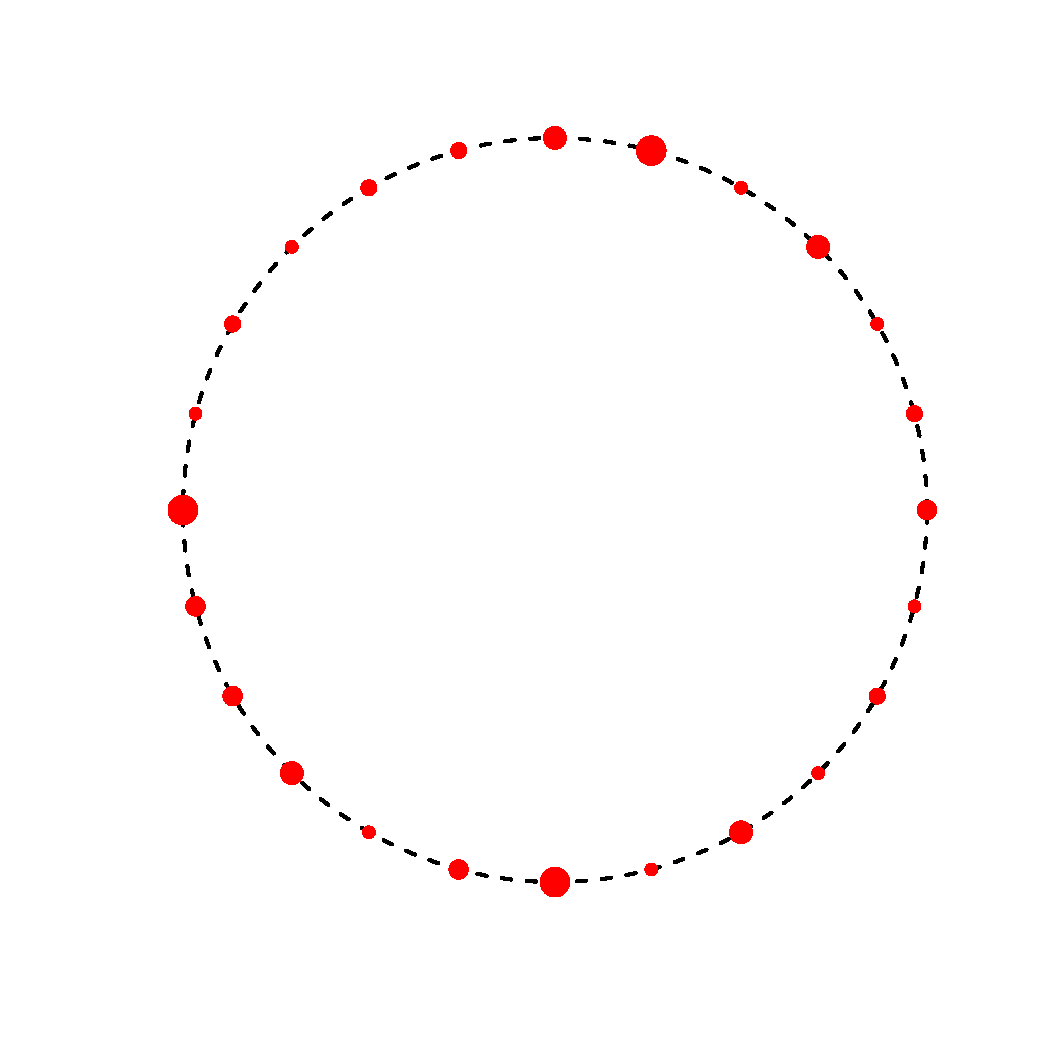
\includegraphics[width=0.5\textwidth]{graphs/process_circle}
	\caption {Random process on a circle at 24 points ($\Delta\lambda = 15^0$), the red dots represent the  observed values at a given time and each point is associated with a random process of it's own.}
\end{figure}

Clearly, each location is correlated with other $n-1$ locations and $C(\theta) = C(-\theta)$ the variance-covariance matrix $\Sigma$ is circulant. We use singular value decomposition (SVD) and obtain the correlated data $\utilde{X}$ on a circle as follows, 

% 
% \begin{eqnarray*}
% 	\Sigma &=& circ(C(0),C(\delta), C(2\delta), \cdots, C((N-1)\delta), C(\pi),  C((N-1)\delta), \cdots, C(\delta)) \\
% 	&=& \left(\begin{array}{ccccccc}
% 	C(0)      & \cdots & C((N-1)\delta ) & C(\pi) &  C((N-1)\delta ) & \cdots & C(\delta) \\
% 	C(\delta) & \cdots & C((N-2)\delta) & C((N-1)\delta) &  C(\pi)  & \cdots & C(2\delta) \\
% 	C(2\delta) & \cdots & C((N-3)\delta) & C((N-2)\delta) &  C((N-1)\delta) & \cdots & C(3\delta)\\
% 	\vdots    & \vdots  & \vdots  & \vdots  & \vdots  & \vdots  & \vdots  \\
% 	C(\delta) & \cdots & C(\pi) &  C((N-1)\delta) & C((N-2)\delta)  & \cdots & C(0) 
% 	\end{array} \right) \\
% 	&=& Q\Lambda Q^T,
% \end{eqnarray*}
% 


\[
	\utilde{X} = \Sigma^{1/2}*Z = Q\Lambda^{1/2}Q^T*Z,  
\]

where  $\Lambda=\{\lambda_1, \lambda_2,\cdots,\lambda_n\}$ and $Q=\{\psi_1, \psi_2,\cdots,\psi_n\}$ are eigen values and eigen vectors of the circulant matrix respectively and $Z\sim N(\utilde{0},1_{n})$.

%-------------------------------------%
\subsection{Covariance estimator comparison} 
%-------------------------------------%

% \beq\label{cov:circle1}
% C(\theta) = \frac{1}{n_L} \sum_{i=1}^{n_L} (X(a_i+\theta)\cdot X(a_i))-(\overline{X(a)})^2
% \eeq

	      In general the covarince estimator (\ref{covarince_estimator}) on a circle is biased, with a bias of $var(\bar{X})$. In order to make things simple we set $C_1, a = 1$ and when $\alpha = 0.5$ $c_0 \ge \int_0^\pi(\theta)^{0.5} \sin \theta d \theta$, from Fresnel intergal it can be shown that $c_0 \ge 2.4353$. Now we compare the covariance estimator (empirical) to it's theoretical covariance given by \ref{exp_cov} and \ref{power_cov}. We computed the MOM estimator $\hat{C}(\theta)$ with 48 gridded observations on the circle from 500 simulations.
	      	      
	      \begin{figure}[H]
	      	\label{covarince_circle}
	      	\centering
	       	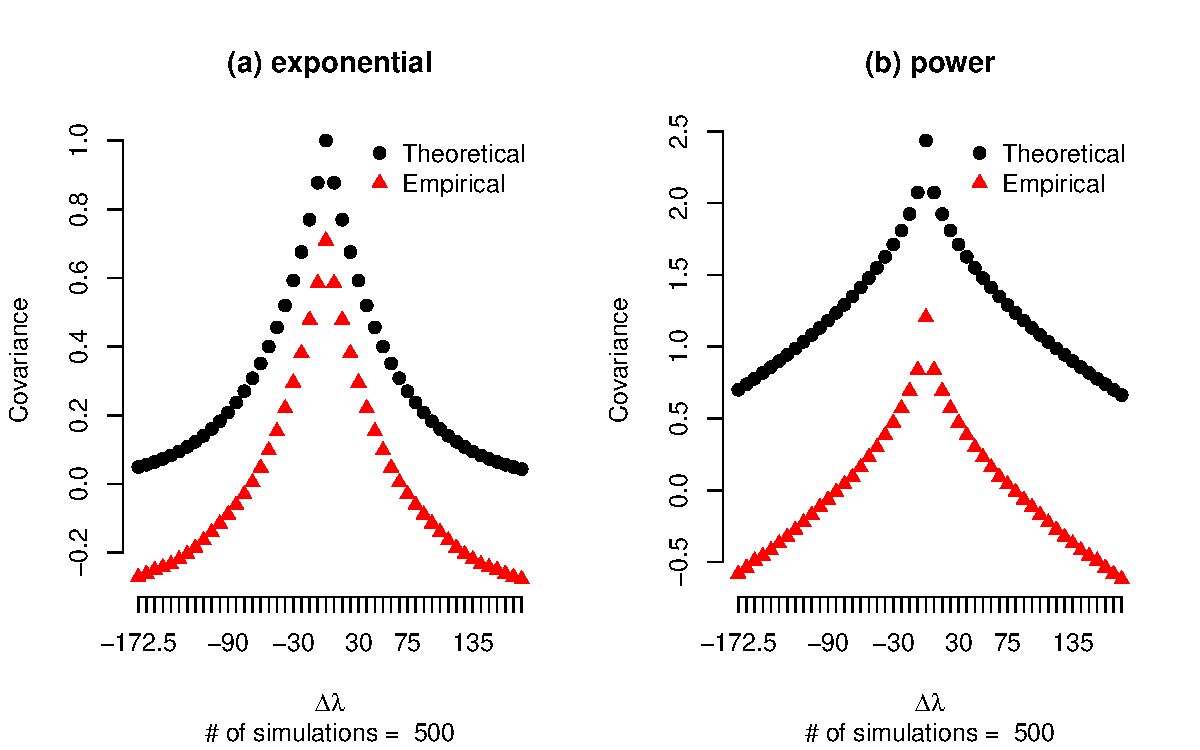
\includegraphics[width=0.9\textwidth]{graphs/covarince_circle}
	      	\caption {Theoretical and empirical covariance (with bias) comparison on a circle, it is easy to notice the bias in both covariance models}
	      \end{figure}

	      {\bf Remark 1:} The shift between theoretical and empirical values is equal to $a_0$ and from $a_0 = \frac{1}{\pi}\int_0^\pi C(\theta)d\theta$ we can obtain
	      
\begin{eqnarray*}
	    \mbox{exponential : }  	a_0 &=& \frac{C_1}{a\pi}(1 - e^{-a\pi}) \\
	    \mbox{power : }  	a_0       &=& c_0 - \left(\frac{\pi}{a}\right)^{\alpha}\frac{1}{\alpha + 1}
\end{eqnarray*}

	      Now consider the following covariance function, after subtracting $a_0$ from $C(\theta)$.
	      \[
	      	D(\theta) = C(\theta) - a_0.
	      \]
      
        If the new covariance function $D(\theta)$ was used to generate the data on a circle then the covariacne estimate converge to the theoretical value. In other words if the process is a zero mean process the covariance estimator given by \ref{covarince_estimator} is unbiased ($i.e. Var(\bar{X}) = 0$) hence we will get a perfect match between theoretical and empirical values.
        
	      % \beq \label{cov:circle1}  
	      % C(\theta) = \frac{1}{n_L} \sum_{i=1}^{n_L} (X(a_i+\theta) \cdot X(a_i)) 
	      % \eeq
	      	      
	      \begin{figure}[H]
	      	\centering
	      	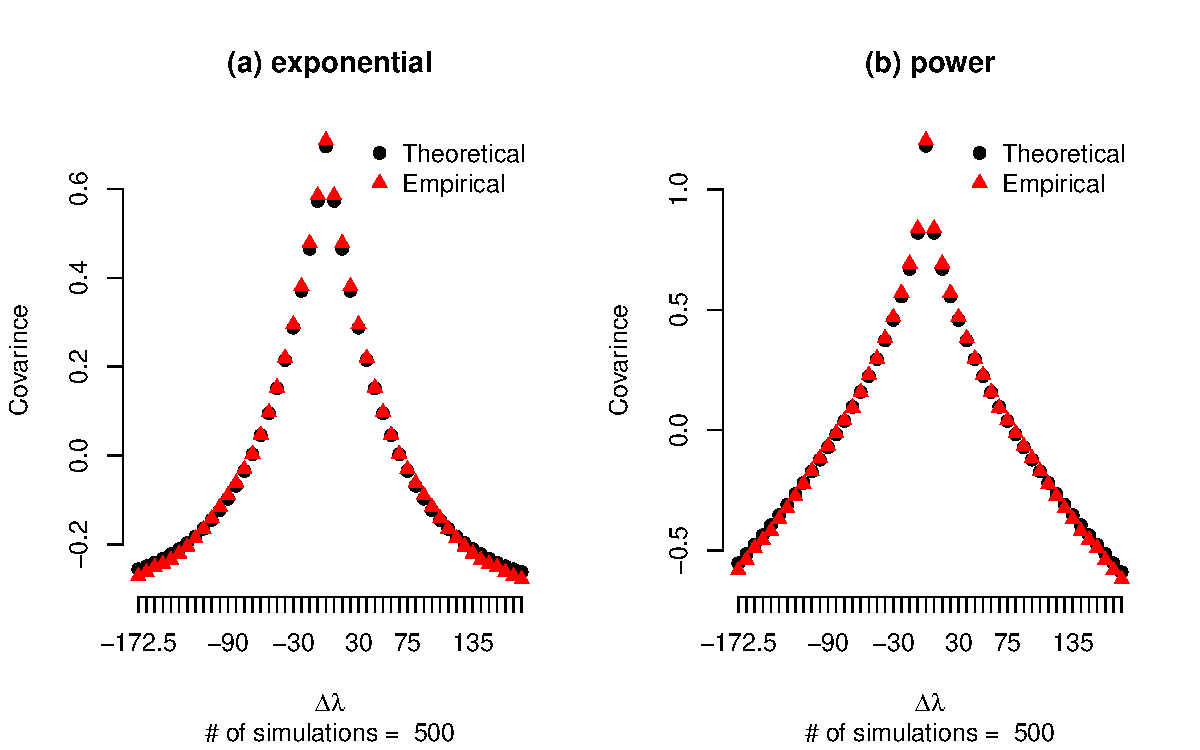
\includegraphics[width=0.9\textwidth]{graphs/covarince_circle_remove_a0}
	      	%graph from data genaration summary doc line 194 
	      	\caption {Theoretical and empirical covariance comparison on a circle using the covariance function $D(\theta)$.}
	      \end{figure}
	      	      

{\bf Remark 2:} The covariance estiamtor is biased and the biasness will approach to $a_0$. When covariance function is unknown the biaseness $a_0$ is also known and the biasness cannnot to estimated (cannot find the variance of $\bar{X}$) from one circle, however as discussed above if multiple $i.i.d.$ copies on the same circle were available then one can estimate $a_0$ {\em i.e.} $\hat{a} = var(\bar{X})$ and substract $\hat{a_0}$ form the MOM estimator as given below,

\[
\hat{C}(\Delta \lambda) = \left( \frac{1}{n}\sum_{i = 1}^n (X(t_i + \Delta \lambda) - \bar{X})(X(t_i) - \bar{X}) \right) -  \hat{a_0}
\]


	\begin{figure}[H]
	 \centering
	 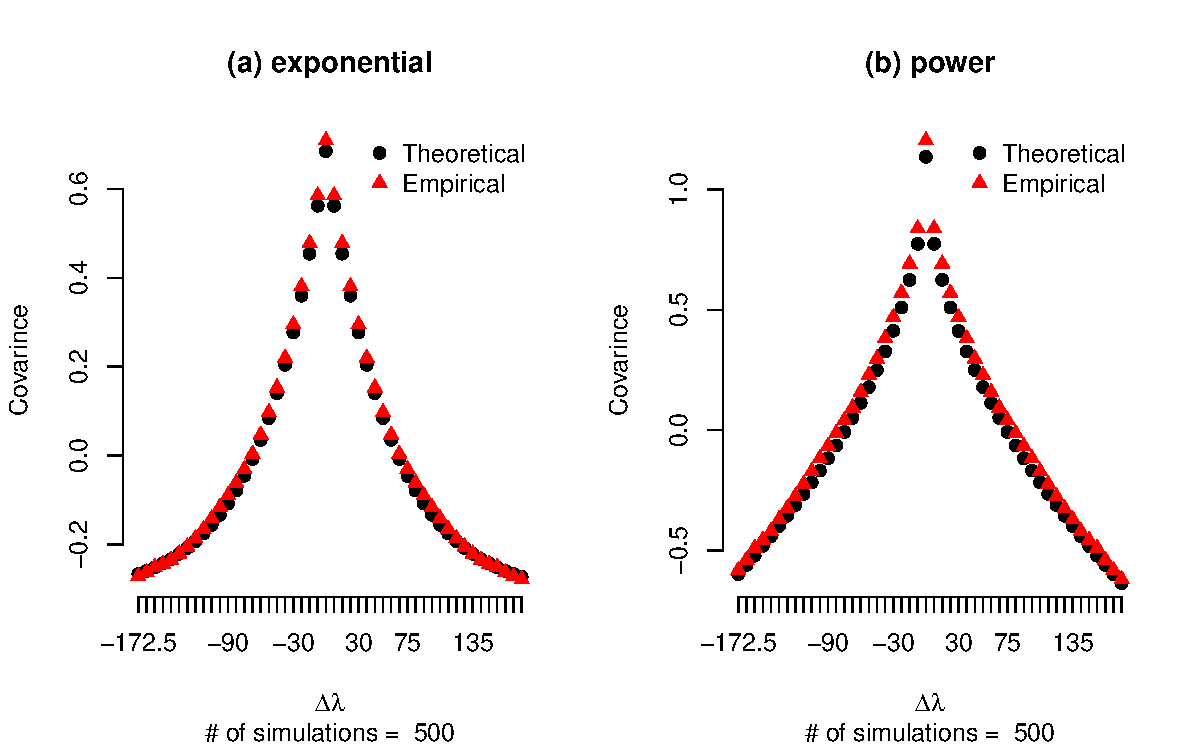
\includegraphics[width=0.9\textwidth]{graphs/covarince_circle_estimate_a0}
	 %graph from data genaration summary doc line 194 
	 \caption {Theoretical and empirical covariance comparison on a circle, after removing $\hat{a_0}$ from the}
	 \end{figure}
	      

	      	      
%-------------------------------------%
\subsection{Variogram estimator comparison} 
%-------------------------------------%

In general the variogram estimator in the case of a is unbiased but not consistent. When the random process on a circle is isotropy the semi variogram is given by 

\[ 
\gamma(\theta) = C(0) - C(\theta),
\]

the theoretical variogram based on exponential and power covariance functions can be given in the following form,   

\begin{eqnarray*}
	\mbox{exponential : }\gamma(\theta) &=& C(0) - C(\theta) = C_1(1-e^{-a|\theta|}) \\
	\mbox{power : } \gamma(\theta) &=& C(0) - C(\theta) = (|\theta|/a)^{\alpha}
\end{eqnarray*}sd

We computed the variogram estimator $\hat{\gamma}(\theta)$ with 48 gridded observations on the circle from 500 simulations since there is no bias varigram estimator is a better fit between theoretical and empirical values compared to covariance estimate.


\begin{figure}[H]
	\centering
	%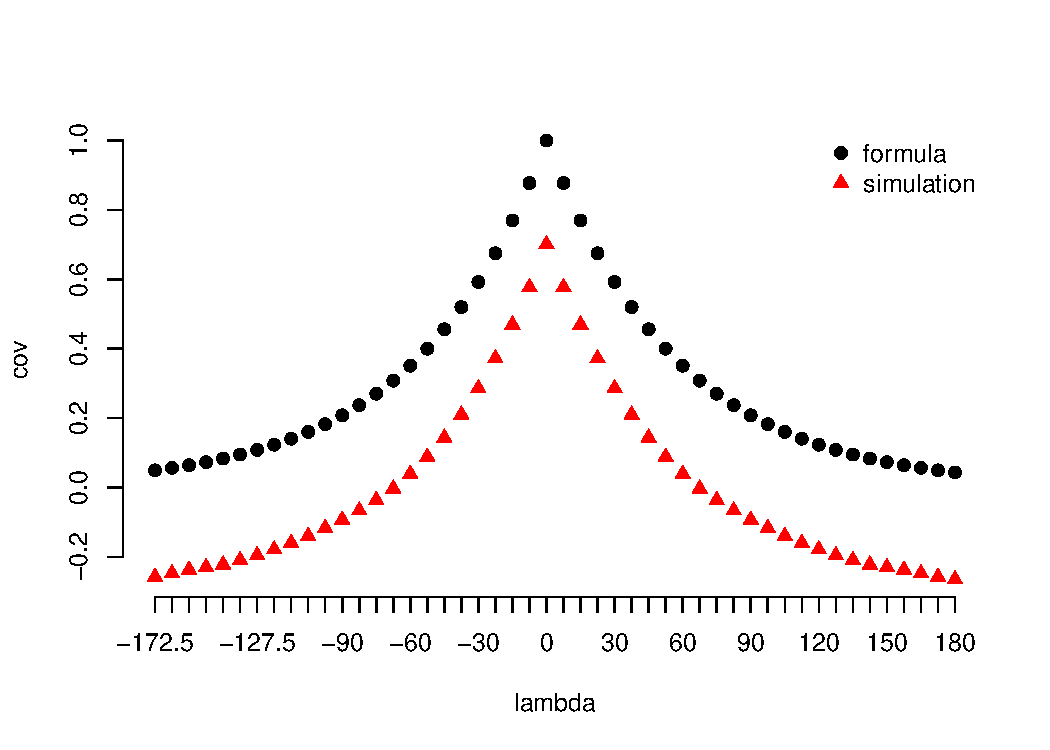
\includegraphics[width=0.65\textwidth]{graphs/Summary-covarince_circle_1}
	%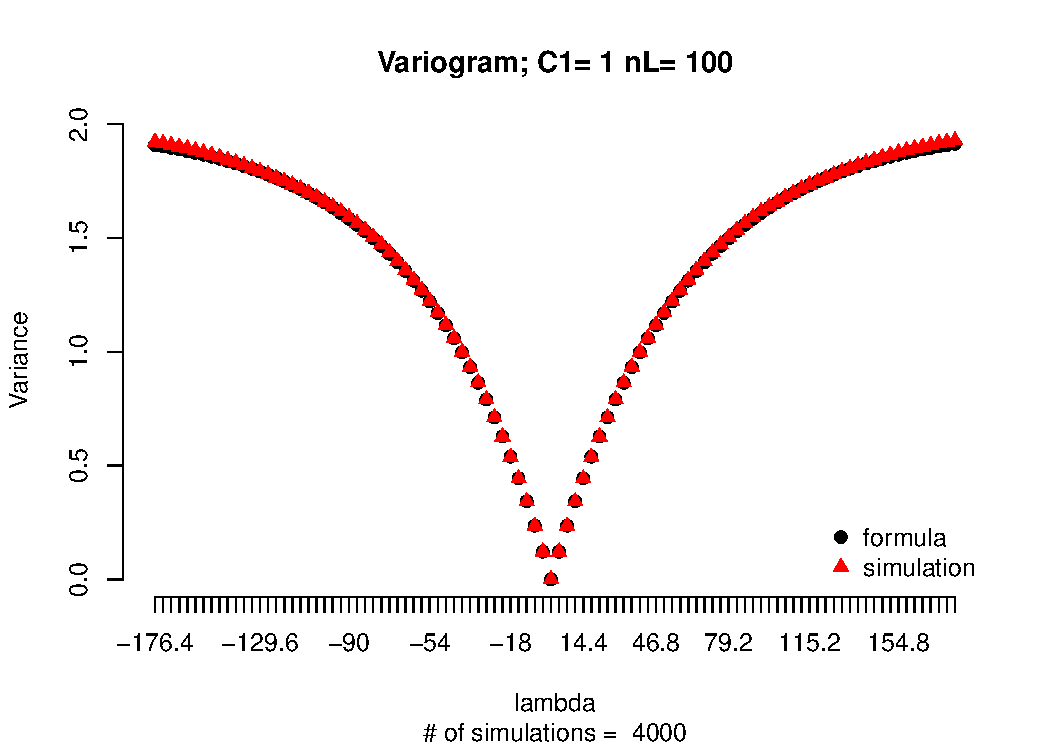
\includegraphics[width=0.65\textwidth]{graphs/variogram_plot_4000}
	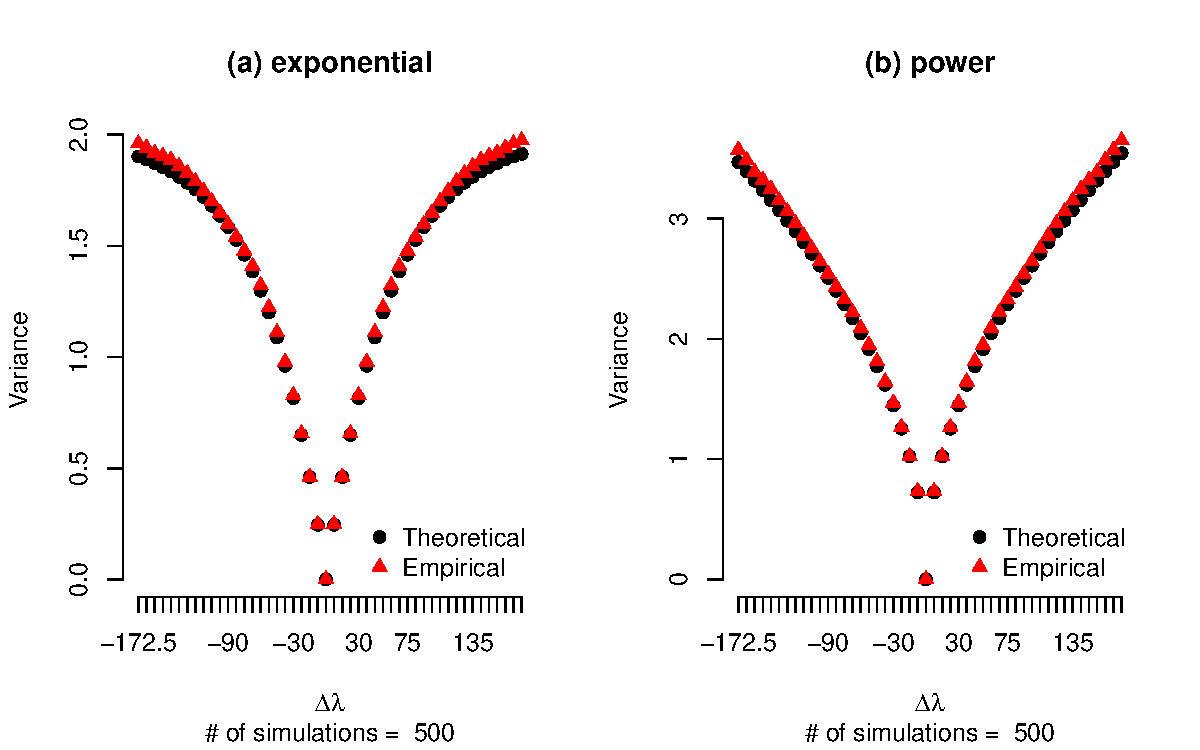
\includegraphics[width=0.9\textwidth]{graphs/variogram_plot_500}
	%graph from data genaration summary doc line 177 
	\caption {Theoretical and empirical comparison for variogram on a circle}
\end{figure}





